\chapter{Desarrollo}

\section{Qu\'{e} se ha hecho}
Se ha desarrollado una aplicaci\'{o}n que dados unos datos organizados
de cierta manera permite la visualizaci\'{o}n de los mismos y
la selecci\'{o}n de unos rangos para guardar y especificar que en ese rango de tiempo
est\'{a} sucediendo una acci\'{o}n determinada, ya sea un Paso o una Situaci\'on.

Los datos de entrada representan Observaciones y Propiedades. Cada observaci\'{o}n tiene una serie
de propiedades que son las que se visualizan. Estos datos, cuando fueron capturados, puede
que tengan uno o varios v\'{i}deos asociados. La visualizaci\'{o}n de los v\'{i}deos es completamente
optativa, y en caso de visualizarlos, van sincronizados con los gr\'{a}ficos a partir del instante que el 
usuario diga.

Es decir, en cada gr\'{a}fico habr\'{a} una l\'{i}nea de progreso para que sea f\'{a}cil determinar en que ciclo
de simulaci\'{o}n estamos \footnote{Un ciclo de simulaci\'{o}n es la unidad de tiempo elegida para la captura de datos, no
    necesariamente es un segundo.}.

Una vez hemos determinado cual es el problema a resolver, se hace necesario tomar ciertas decisiones.
Desde un principio se sab\'ia que hab\'ia que programar en un entorno Windows, utilizando Visual Studio 2013.
La raz\'on de esta decisi\'on fue que el proyecto actual est\'a desarrollado utilizando Windows Forms, y el 
director del proyecto coment\'o que exist\'ia una intenci\'on de portarlo a WPF.

Pese a conocer esa intenci\'on, hubo que valorar qu\'e merec\'ia m\'as la pena, si utilizar WPF, una tecnolog\'ia moderna
en la que Microsoft est\'a poniendo todo su empe\~no, o bien Windows Forms, que es un viejo conocido del desarrollo
.NET con un camino muy largo de desarrollo.

Para decidir de la manera m\'as objetiva posible, se confeccion\'o la tabla \ref{ComparativaWPF} en la que se sit\'uan 
las caracter\'isticas de cada tecnolog\'ia. La tabla es una elaboraci\'on propia confeccionada a partir de una comparativa
online \cite{WPFvsWinForms:Comparative}.

\begin{table}[H]
	\begin{center}
		\rowcolors{1}{lightgray}{} %\rowcolors{<starting row index>}{<odd row color>}{<even row color>}
		\begin{tabular}{|p{5cm} | p{4cm} | p{4cm}|}
			\rowcolor{darkgray}                         & \color{white}Windows Forms               & \color{white}WPF \\
			Formularios y controles                     & Si                                       & Si \\
			Documentos en pantalla                      & Si                                       & Si \\
			Documentos de formato fijo (XPS, PDF)       & No                                       & Si \\
			Im\'{a}genes                                & No                                       & Si \\
			V\'{i}deo y audio                           & No                                       & Si \\
			Gr\'{a}ficos 2D                             & No                                       & Si \\
			Gr\'{a}ficos 3D                             & No                                       & Si \\
			Interfaz compatible con altas resoluciones  & No, basada en BMP                        & Si, basada en vectores \\
			Creaci\'{o}n de la interfaz                 & Arrastrando y soltando los elementos     & Interfaz declarativa tipo XML \\
			Multilenguaje                               & Mediante archivos de recursos, f\'{a}cil y bien documentado & Mediante DLLs sat\'{e}lite, poco documentado y las herramientas aun no est\'{a}n listas para un entorno de producci\'{o}n. \\
			\hline
		\end{tabular}
	\end{center}
	\caption[Comparativa Windows Forms y WPF]{Comparativa Windows Forms y WPF}
	\label{ComparativaWPF}
\end{table}

C\'omo puede observarse, Windows Forms se ha quedado obsoleto para un desarrollo de aplicaciones moderno.
Pese a todo, WPF, tiene algunos puntos d\'ebiles. Entre ellos, el soporte multilenguaje, y que es un proyecto
mucho menos maduro, ya que fue lanzado en 2006 junto con .NET Framework 3 \cite{WPF:Overview}. Windows Forms,
por su parte se present\'o junto con la primera version de .NET Framework, en 2002.

Esta elecci\'on condiciona el resto de decisiones que fueron tomadas, ya que las bibliotecas gr\'aficas
de Windows Forms no son compatibles con WPF. Existe una capa de compatibilidad en la que es posible embeber dentro
de un host WPF un control Windows Forms, pero no es recomendable, ya que no deja de ser una capa de compatibilidad y
no es posible sacarle toda la potencia a Windows Presentation Foundation.

Una de las primeras decisiones que se tomaron, y adem\'as sin demasiado debate, fue que tipo de interfaz se deseaba.
Se eligi\'o una interfaz tipo IDE, con ventanas acoplables, tal y como se ha detallado en el cap\'itulo de Antecedentes.

En este caso en concreto no hubo que buscar mucho, ya que no hay mucho donde elegir. La biblioteca seleccionada
fue AvalonDock.

AvalonDock es una biblioteca escrita \'integramente para WPF, con soporte para MVVM. Permite todo lo que se espera
de un proyecto como ese: Ventanas acoplables a los lados, mover pesta\~nas etc, fue curioso que durante desarrollo se descubri\'o
un bug en el software.

Dicho bug, lanzaba una excepci\'on cuando un elemento ``acoplable", que ten\'ia un Men\'u superior, al ponerlo
en una pesta\~na, al cambiar de pesta\~na fallaba. El bug ya estaba reportado, pero aun as\'i se le proporcion\'o
al desarrollador m\'as informaci\'on sobre el bug \footnote{\url{https://avalondock.codeplex.com/discussions/429063}}, y a d\'ia de hoy
sigue sin estar resuelto.

Antes de explicar como es la interfaz que se ha dise\~nado, primero hay que saber como trabaja internamente
AvalonDock y como se usa para poder crear esas pesta\~nas y ventanas acoplables.

Explicado de manera muy sencilla, AvalonDock se compone de cuatro partes principales: el \emph{DockingManager},
el \emph{LayoutPanel}, el \emph{LayoutAnchorablePane}, y el \emph{LayoutAnchorable}.
Tambi\'en tiene otros elementos pero no han sido usados en este proyecto.

\paragraph{DockingManager:} Es el n\'ucleo de AvalonDock, donde todos los elementos WPF son a\~nadidos, necesario
siempre para poder trabajar con AvalonDock.

\paragraph{LayoutPanel:} Este elemento organiza todos los hijos, poniendo un separador entre ellos, establecido
usando la propiedad \emph{Orientation}.

\paragraph{LayoutAnchorablePane:} Estos elementos son la clave. Ya que es el panel que permite que los objetos
\emph{LayoutAnchorable} pueden ser arrastrados, puestos en pesta\~nas, lado a lado etc.

\paragraph{LayoutAnchorable:} Estos elementos siempre deben ir dentro de un \emph{Pane}, bien en un \emph{LayoutAnchorablePane}
bien en un \emph{LayoutDocumentPane} que no ha sido explicado. Estos elementos son los que pueden reorganizarse como uno quiera,
anclarse a un lado, poner que se oculten etc. Y dentro pueden tener aquello que se desee.

Por tanto, para tener una instancia funcional de AvalonDock, tendremos que tener un \emph{DockingManager} y un
\emph{LayoutRoot} dentro de ese dockingmanager. Y dentro de ese \emph{LayoutRoot} un \emph{LayoutAnchorablePane}.

Una vez tenemos eso, a\~nadir a un \emph{LayoutAnchorable} un elemento es muy sencillo, no hay mas que a\~nadirlo dentro de la
propiedad Content. Y para a\~nadir ese \emph{LayoutAnchorable} al \emph{LayoutAnchorablePane} hay que a\~nadirlo a la colecci\'on
de hijos. En la Figura \ref{AnadirHijoAvalonDock} se puede ver un ejemplo de como se a\~nade un \emph{UC\_DataVisualizer} a 
AvalonDock.

\begin{figure}[h]
    \begin{lstlisting}[tabsize=2, language=C, numbers=left, showspaces=false, breaklines=true]
    public void addToAnchorablePane(UserControl objectToAdd, string Title)
    {
        UC_DataVisualizer datav = (UC_DataVisualizer)objectToAdd;
        LayoutAnchorable doc = new LayoutAnchorable();
        doc.Title = Title;
        doc.Content = datav;
        mainPanelChartContainer.Children.Add(doc);

    }
    \end{lstlisting}
    \caption[Adici\'on de elemento a AvalonDock]{Adici\'on de elemento a AvalonDock}
    \label{AnadirHijoAvalonDock}
\end{figure}

Una vez conocemos el funcionamiento de AvalonDock, podemos pasar a hablar de la interfaz dise\~nada.
La estructura que se ha dise\~nado es un ``workbench", con un panel lateral en el que se pueden visualizar las observaciones
y propiedades disponibles despu\'es de haber cargado un fichero XML. Cuando se hace doble click sobre un elemento
de ese \'arbol de propiedades y observaciones, el software sabe si se ha pinchado en una propiedad o en una observaci\'on.
Si se quiere saber que sucede cuando se pincha en cada uno de ellos, todo esto est\'a mejor explicado en anexo 
\ref{chap:CasosDeUsoExt} de
Captura de requisitos, en los casos de uso extendidos.

Cuando se cargan los datos que se desean, es decir, que se visualizan, como puede verse en la
Figura \ref{fig:EjemploObservacion} se muestran organizados por observaciones. Y dentro de cada
observaci\'on las propiedades que han sido cargadas. Las ventanas pueden organizarse como se quiera, ponerlas lado a lado,
reordenar las pesta\~nas, colapsarlas a un lateral, dejarlas como ventanas flotantes etc. 
La \'unica limitaci\'on intencionada es que una propiedad no puede acoplarse a una observaci\'on a la que no pertenece,
para evitar confusiones.

\begin{figure}[h]
	\centering
	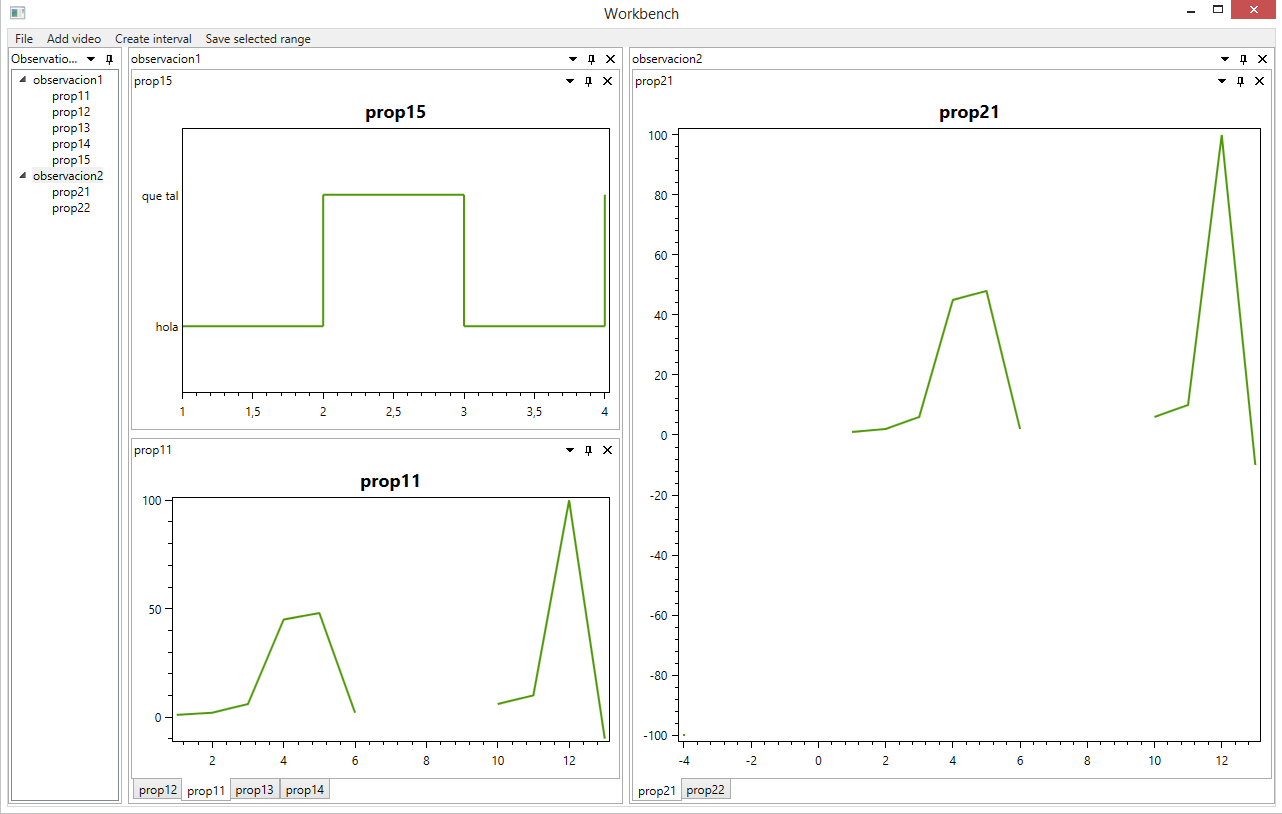
\includegraphics[width=0.9\linewidth]{./Figures/Capturas/EjemploObservacion.PNG}
	\caption{Ejemplo de visualizaci\'on de propiedades}
	\label{fig:EjemploObservacion}
\end{figure}

Despu\'es de escoger el tipo de organizaci\'on de ventanas, era necesario elegir como iban a mostrarse los gr\'aficos en pantalla.
Para el sistema de gr\'aficos no hubo problemas a la hora de encontrar distintas librer\'ias, pero s\'i que fue un 
problema encontrar uno que cumpliera las siguientes caracter\'isticas.

\begin{itemize}
	\item Permitir mostrar gr\'{a}ficos cont\'{i}nuos y discretos, y estos \'{u}ltimos tanto num\'{e}ricos como por categor\'{i}as.
	\item Permitir la selecci\'{o}n de rangos con el rat\'{o}n.
	\item Permitir mostrar el progreso del v\'{i}deo asociado. Bien sin programar la funci\'{o}n o al menos que fuese f\'{a}cilmente programable.
\end{itemize}

Se descartaron todas las bibliotecas de pago, como pueden ser Telerik, SciChart, Visiblox, etc. por ser demasiado caras
y porque se decidi\'o utilizar en la medida de lo posible tecnolog\'ias libres y gratuitas. Entre las bibliotecas
gratuitas, destacaron tres por encima de todas. Las capacidades nativas de WPF,
WPF toolkit, desarrollada por Microsoft, y OxyPlot.

Los gr\'aficos 2D integrados en WPF son muy simples de utilizar, con una est\'etica muy minimalista, de colores planos.
Lamentablemente, la selecci\'on de rangos, y mostrar leyendas en los ejes X e Y no eran tareas triviales, por lo que
se descart\'o al poco de iniciar el desarrollo.

WPF toolkit fue la siguiente librer\'ia en pasar la prueba. Se integra a la perfecci\'on 
en Visual Studio y muestra unos gr\'aficos muy profesionales de una forma
muy simple, pero desafortunadamente, no existe una manera sencilla de seleccionar un rango.

OxyPlot, por su parte, es un proyecto comunitario en constante desarrollo. Con decenas de ejemplos online en su web
oficial fue muy sencillo crear un prototipo funcional con todos los gr\'aficos requeridos, con las leyendas en los ejes
y los t\'itulos. Conseguir la selecci\'on de un rango conllev\'o algo m\'as de tiempo de desarrollo.

Para crear un gr\'afico es tan f\'acil como crear en el XAML un elemento \emph{<oxy:PlotView />} que va a ser el 
elemento que va a contener el gr\'afico. Despu\'es, \'unicamente hay que a\~nadir un \emph{PlotModel}, que es la
clase que contiene tanto los puntos, el titulo del gr\'afico, los ejes etc. Lo mejor en estos casos es un ejemplo.
En la Figura \ref{CreacionPlotModel}, se ve el m\'etodo de creaci\'on de un \emph{PlotModel} para un visualizador de datos
discreto.

\begin{figure}[h]
    \begin{lstlisting}[tabsize=2, language=C, numbers=left, showspaces=false, breaklines=true]
    protected override PlotModel createModel(List<DataPoint> points)
    {
        var plotModel = new PlotModel();
        var functionSeries = new StairStepSeries();
        var categoryAxis = new CategoryAxis();
        
        categoryAxis.Position = AxisPosition.Left;
        categoryAxis.AxislineStyle = LineStyle.Solid;
        categoryAxis.MinorStep = 1;
        categoryAxis.TickStyle = TickStyle.None;
        categoryAxis.Labels.AddRange(Labels);
        plotModel.Axes.Add(categoryAxis);
        functionSeries.Points.AddRange(points);
        plotModel.Series.Add(functionSeries);
        plotModel.Title = Title;
        Points = functionSeries.Points;
        return plotModel;
    }
    \end{lstlisting}
    \caption[Creaci\'on PlotModel]{Creaci\'on PlotModel}
    \label{CreacionPlotModel}
\end{figure}

La selecci\'on de un rango, se hace a\~nadiendo al \emph{PlotModel} un elemento \emph{RectangleAnnotation}.
Para actualizar el valor de inicio y fin de ese rango, hay que suscribirse a tres eventos, ya que una selecci\'on
de rango es la combinaci\'on de tres eventos: hacer click, arrastrar, y dejar de hacer click. Cuando se pincha,
se establece el lugar de inicio de selecci\'on, y mientras se va moviendo el rat\'on, si el bot\'on izquierdo
del rat\'on est\'a presionado, entonces se va actualizando el rango seleccionado. Y cuando se deja de pinchar,
termina el proceso.

En los primeros prototipos, en cada gr\'afico pod\'ia seleccionarse un rango diferente, pero era algo inconsistente, ya
que cuando llegase la hora de guardar los rangos, ¿Cual se usar\'ia? Por lo que fue necesario continuar un poco con la 
investigaci\'on para ver como podr\'ia un hijo notificar a su padre de que ha cambiado, para que ese padre notifique a todos
sus hijos para sincronizarse. Recu\'erdese,
que los elementos est\'an dispuestos en forma de \'arbol, de 
la pantalla principal cuelgan las observaciones y el
contenedor de v\'ideos,
y de cada observaci\'on sus hijos son los gr\'aficos que
representan las propiedades, y del contenedor de v\'ideos, sus hijos
son los propios v\'ideos. Para mayor detalle ver el cap\'itulo de An\'alisis y dise\~no.

La primera aproximaci\'on, y posiblemente la peor de todas, era realizar un \emph{polling}, es decir, cada, por ejemplo, 60 ms,
preguntar a cada elemento si ha cambiado, y si alguno lo ha hecho, utilizar ese valor para poner ese rango en los dem\'as 
gr\'aficos. Este enfoque, tiene diversos problemas, pese a que los gr\'aficos est\'an guardados en \'arboles rojo-negro
\footnote{\url{https://www.cs.auckland.ac.nz/~jmor159/PLDS210/red\_black.html}}
\footnote{\url{https://www.cs.princeton.edu/courses/archive/fall08/cos226/lectures/10BalancedTrees-2x2.pdf}}, que son
unos \'arboles binarios autobalanceables,
no tiene sentido recorrer el \'arbol constantemente, y si se encuentra un elemento, habr\'ia que recorrer cada observaci\'on cargada,
y para cada observaci\'on todas las propiedades cargadas actualmente. Eso,
conllevar\'ia un coste de O(2*n*m) siendo ``n" \ el n\'umero de observaciones cargadas y ``m" \ el n\'umero de propiedades.

La otra soluci\'on, es implementar la interfaz \emph{INotifyPropertyChanged}. Utilizando esta interfaz, se expone un 
nuevo evento, llamado \emph{PropertyChanged} al que otros objetos se pueden suscribir para estar a la escucha. 

De esta manera, cada vez que se a\~nada un nuevo gr\'afico, el contenedor de gr\'aficos se suscribe a ese evento para todos
sus hijos. De esta manera, cuando el rango seleccionado cambie, ser\'a ese hijo el que notifique al padre, que iniciar\'a
el proceso de sincronizado, tanto con sus hijos como con sus hermanos (el resto de observaciones cargadas).

Para la visualizaci\'on de v\'ideos no hubo mucho problema, y se utilizaron los
propios componentes de WPF, que cumpl\'ian todas las necesidades.

Por su parte, cargar los datos no fue demasiado problema una vez se decidi\'o cual iba a ser el formato de los
ficheros XML.

Se barajaron dos posibilidades. La primera, que por cada instante de simulaci\'on se guardaran las observaciones
que est\'an teniendo lugar, y los valores de las propiedades que tienen en ese instante, tal y como
se puede ver en la Figura \ref{Estructura XML1}.

Este formato, a la vista parece bueno, ya que se pordr\'ia construir los gr\'aficos instante a instante,
todos a la vez. Pero, ¿Y si se quiere obtener el valor de una propiedad en concreto para mostrar todo 
el gr\'afico de golpe? No se obtiene de manera directa, ya que habr\'ia que ciclar a trav\'es de todos los nodos
instante, y a trav\'es de todos los nodos observaci\'on, buscando la propiedad deseada.

Tambi\'en hay que tener en cuenta, que en distintas observaciones puede haber propiedades que tengan el mismo nombre, 
aumentando la complejidad de la consulta LINQ (m\'as adelante se hablar\'a de este tema).

\begin{figure}[h]
    \lstinputlisting[tabsize=2, language=XML, numbers=left]{./Attachments/Adjunto1.xml}
    \caption[Estructura XML 1]{Estructura XML 1}
    \label{Estructura XML1}
\end{figure}

La segunda opci\'on barajada, toma un enfoque distinto., tal y como se puede
ver en la Figura \ref{Estructura XML2}. Los datos se agrupan por observaci\'on, con las observaciones teniendo sus propiedades,
y estas \'ultimas sus instantes. De esta manera, de un simple vistazo podemos determinar todos los valores que va a tomar
una propiedad de una observaci\'on en concreto, sin ning\'un tipo de consulta compleja.
En el nodo \emph{<data>} se ha a\~{n}adido un nuevo atributo \emph{instantLength} que 
determina la longitud de un instante.

Por ejemplo, en la propiedad \emph{prop14} se ve que los instantes no son consecutivos, por lo que el sistema sabe que el 
gr\'{a}fico no debe ser cont\'inuo en ese punto, es decir, desde el punto (1, 4) no debe unirse al 
(3, 5). Esto es \'{u}til para saber si una propiedad esta sucediendo o no.

\begin{figure}[h]
    \lstinputlisting[tabsize=2, language=XML, numbers=left]{./Attachments/Adjunto2.xml}
    \caption[Estructura XML 2]{Estructura XML 2}
    \label{Estructura XML2}
\end{figure}

Otro de los problemas fundamentales que se tuvieron, fue como guardar los datos. Debido a que de momento MIPS va a ser completamente independiente, hab\'ia que buscar una manera de compartir los datos
que implicara el menor n\'umero de cambios posibles en ULISES.

Se barajaron varias posibilidades, como por ejemplo, las bases de datos relaciones, pero este sistema requerir\'ia
de una estructura compleja para guardar unos datos bastante sencillos. Ya que del modelo de dominio, se infiere que m\'inimo,
iba a haber 4 tablas para poder guardar los datos correctamente. Adem\'as, los datos no iban a ser f\'acilmente 
comprensibles por humanos, ya que ser\'ian un amasijo de n\'umeros guardados en tablas que ser\'ian dif\'iciles de
relacionar entre ellas de manera sencilla.

Es por ello que se valor\'o la posibilidad de utilizar las bases de datos no relacionales, que est\'an tan de moda
\'ultimamente. Concretamente, el producto sometido a pruebas fue MongoDB. Es una base de datos NO-SQL en la que los
datos se guardan en formato de ``documentos", no tablas. Internamente, se guardan en formato BSON, que no deja de ser
un JSON binario \footnote{Especificaci\'{o}n JSON: \url{http://json.org/}}. Ofrece un gran rendimiento, adem\'as
de unos datos mejor organizados para esta tarea, con elementos que tienen arrays, y cada elemento atributos etc.

Finalmente se opt\'o por descartarlo tambi\'en, ya que a\~nad\'ia mayor complejidad, ``oscuridad" \ y requisitos a la 
implementaci\'on. Ya que habr\'ia que tener instalada una base de datos MongoDB, as\'i como los conectores para
C\#.

As\'i que se decidi\'o ir por el camino de en medio y elegir un est\'andar que no requiriera de software adicional,
que fuese soportado de manera nativa por el lenguaje de programaci\'on y adem\'as f\'acilmente comprensible por
humanos. El elegido fue XML m\'as la biblioteca LINQ To XML incluida por defecto en .NET Framework. 

XML es un est\'andar recomendado por la W3C \cite{XML:Specification}, y la versi\'on actual es la 1.0 quinta edici\'on.
Por si mismo, XML no aporta ning\'un tipo de ventaja adicional respecto a las otras opciones, excepto el que no se
requiere de software adicional para compartir los datos de una aplicaci\'on a otra, y que
se pueden crear esquemas XSD para validar esos datos de manera muy sencilla. 
Lo que realmente marca
la diferencia es LINQ To XML.

LINQ To XML es una extensi\'on de la biblioteca LINQ (Language Integrated Query), que permite hacer consultas
similares a SQL a estructuras de datos .NET. 

En el ejemplo de la Figura \ref{Consulta LINQ}, extra\'ido de mi propio c\'odigo, se obtienen las propiedades de
una determinada observaci\'on.
Concretamente, este c\'odigo se ha utilizado a la hora de cargar el \'arbol lateral
de observaciones y propiedades.

\begin{figure}[h]
	\begin{lstlisting}[tabsize=2, language=C, numbers=left, showspaces=false, breaklines=true]
		internal List<string> getPropertiesOf(string observation)
        {
            List<string> listProperties = null;
            
            IEnumerable<XElement> properties =
                from prop in xml.Descendants("property")
                where (string)prop.Parent.Attribute("name") == observation
                select prop;
            
            listProperties = addElements(properties);
            return listProperties;
        }
	\end{lstlisting}
	\caption[Consulta LINQ]{Consulta LINQ}
	\label{Consulta LINQ}
\end{figure}

Otras de las cosas que se implementaron a \'ultima hora fue la posibilidad de guardar m\'ultiples
intervalos en un mismo Paso o Situaci\'on, ya que en palabras del director del TFG: ``No todo lo que est\'a 
relacionado sucede \'unicamente durante un intervalo de tiempo". Para hacer frente a esta nueva funcionalidad
hubo dos enfoques principales. El primero de ellos, consist\'ia en que cada vez que se le diera a guardar
intervalo, el software preguntara si se quer\'ian a\~nadir intervalos mas tarde. Cuando se pinchara que no
se mostrar\'ia el di\'alogo de guardar y se guardar\'ia a disco.

La otra opci\'on, era separar las dos acciones, por un lado, crear los intervalos, y por otro lado guardar a disco.
Finalmente se utiliz\'o la segunda manera porque se cree de que es m\'as intuitivo tener dos acciones separadas
que se sabe bien que realiza cada una, con un flujo de trabajo claro, a tener una \'unica acci\'on, que dependiendo
de la acci\'on del usuario haga una cosa u otra. 

Una vez elegido el m\'etodo de guardado de datos y teniendo en mente que
deben poder guardarse m\'ultiples intervalos en un mismo paso o situaci\'on, se llego a la tesitura de elegir una estructura de guardado para el XML.

Como no se quería añadir complejidad, se utilizó la misma estructura que
para la de cargado, pero añadiendo un nodo \emph{<interval>}. Lo mejor, es un
ejemplo, tal y como puede verse en la figura \ref{EstructuraGuardado}.

\begin{figure}[h]
    \lstinputlisting[tabsize=2, language=XML, numbers=left]{./Attachments/guardado.xml}
    \caption[Estructura de guardado]{Estructura de guardado}
    \label{EstructuraGuardado}
\end{figure}

Para poder determinar si los ficheros XML son v\'alidos se han creado dos 
esquemas XSD. La ubicaci\'on de los ficheros XSD se especifican en el fichero 
de configuraci\'on del programa. Por defecto la ubicaci\'on de los esquemas es 
en la carpeta ra\'iz del software, dentro de una carpeta ``schemas".

Una cosa interesante y que adem\'as no se ped\'ia desde el principio, era si 
ten\'ia sentido implementar procesamiento paralelo o procesos en segundo plano. El 
procesamiento paralelo finalmente no tiene sentido implementarlo ya que no hay tareas
que puedan separarse en subtareas para que cada ``trabajador" \ pueda procesar por su
cuenta. En cambio, al no conocerse el tama\~no m\'aximo de entrada, se ha decidido
implementar un \emph{BackgroundWorker} a la hora de crear un intervalo, y a la hora
de guardar en disco el paso o la situaci\'on.

Se ha tomado esta decisi\'on porque si el guardar los datos se hace en el hilo principal
de ejecuci\'on, dependiendo de la cantidad de datos, podr\'ia bloquear la interfaz y
de esta manera el software es mucho m\'as escalable. Bien es
verdad que un procesador moderno es capaz de procesar unos 50 millones de operaciones por
segundo, y no se cree que la entrada, ni la salida vaya a ser tan grande.

A la hora de cargar datos, no se ha implementando el \emph{BackgroundWorker}
porque en la aplicaci\'on no se puede realizar ninguna acci\'on hasta que los datos est\'an 
listos. Pese a todo, al cargar el XML no se cargan todos los datos, sino que se obtienen \'unicamente
los nombres de las propiedades y las observaciones. Los datos en si se cargan bajo demanda, para optimizar la memoria
utilizada del propio software haci\'endolo mas \'agil al mismo tiempo, ya que de esta manera el software no
tiene que preocuparse de que datos est\'an cargados y cuales no, ya que todo aquello que est\'a cargado debe
procesarse.

En cuanto a las cuestiones de dise\~no, tal y como se ha contado previamente en el cap\'itulo
de An\'alisis y dise\~no se ha realizado de manera iterativa, mejorando el dise\~no sprint tras sprint. Se tom\'o esta decisi\'on siguiendo los principios de Scrum, concretamente
el principio emp\'irico \cite{SCRUM:Empiricism}, es decir, que se basa 
en la experimentaci\'on y no
en la planificaci\'on. Por tanto 
se acepta que un problema no puede ser completamente entendido o definido desde un primer
momento, ya que en fases m\'as avanzadas del proyecto, cuando se tenga m\'as experiencia,
se ver\'a que muchas de las cosas dise\~nadas previamente est\'an mal o se pueden
mejorar en gran medida.

Por ejemplo, al principio, la clase \emph{GraphicsActions} conten\'ia una lista con todos los 
\emph{UC\_DataVisualizer}. Este
acercamiento se eligi\'o al principio ya que era el m\'as simple para conseguir el objetivo del mes: mostrar datos.

Posteriormente, se hizo necesario guardar tambi\'en los \emph{UC\_ChartContainer}, ya que las propiedades estaban agrupadas por
observaci\'on. Por lo tanto \emph{GraphicsActions} pas\'o a tener un \emph{HashMap} teniendo como clave el nombre de la 
observaci\'on
y como contenido una lista de \emph{UC\_DataVisualizer}. Pero ese dise\~no entra en conflicto con uno de los principios
SOLID que ya fueron explicados. Por lo que \emph{GraphicsActions} ahora es un repositorio de 
\emph{UC\_ChartContainer},
y cada \emph{UC\_ChartContainer} contiene una lista de los\emph{ UC\_DataVisualizer} que 
pertenecen a esa observaci\'on y un \emph{HashSet}
con los nombres de las propiedades, para poder obtener en tiempo constante si ya estaban cargados, ya que solo se pueden cargar
una \'unica vez.

En la \'ultima iteraci\'on, se decidi\'o sustituir el \emph{HashSet} y la lista por un \'arbol rojo-negro. Ya que permite
inserci\'on, b\'usqueda y eliminaci\'on en tiempo O(ln n) frente al O(n) de las listas. 
Adem\'as un \'arbol rojo negro, s\'olo permite que existe una vez el mismo 
objeto en el \'arbol.

\section{Gesti\'{o}n del c\'{o}digo fuente}
Hasta ahora no se ha hablado de algo que bien no es parte del desarrollo, pero que igualmente es importante.

Hoy en d\'ia, todo proyecto debe tener alg\'un tipo de gesti\'on del c\'odigo fuente, para evitar p\'erdida de datos, 
poder volver a versiones anteriores y tener una mejor noci\'on de que se ha cambiado si es un proyecto colaborativo.

En este caso, al ser un proyecto realizado por una \'unica persona, parec\'ia razonable utilizar alg\'un otro tipo
de sistema. Ya que Git, CVS o Subversion son piezas de software muy potentes y usadas a gran escala, pero tienen
una curva de aprendizaje bastante pronunciada.

Por tanto se valor\'o la posibilidad de utilizar Dropbox como sistema de gesti\'on y sincronizado del c\'odigo fuente.
Pero los problemas no tardaron en aflorar con cuestiones del tipo:

¿Qu\'e pasar\'ia si se quiere volver a una versi\'on de hace 20 d\'ias? ¿C\'omo se crea un trabajo derivado a partir
de una versi\'on concreta? Por lo que finalmente se decidi\'o usar Git, ya que incluso con la curva de aprendizaje,
es una herramienta muy potente y \'util, en la que se puede ver f\'acilmente qu\'e se hizo cierto d\'ia, o volver sin 
ning\'un problema a lo que se hizo ayer, o a lo que se hizo el primer d\'ia de proyecto.

Crear una nueva rama de desarrollo a partir de cualquier versi\'on es muy \'util y pr\'actico, por ejemplo, para
realizar pruebas experimentales sin romper el trabajo estable que se ha realizado hasta el 
momento, o para arreglar alg\'un bug de una versi\'on que ya est\'a en producci\'on. 
Tambi\'en ha sido fruto de diversos problemas, pero nada que el manual 
oficial o StackOverflow no pudieran
resolver en unos minutos.

\section{Creaci\'{o}n de la documentaci\'{o}n}
Aunque esta secci\'{o}n pueda parecer una elecci\'{o}n obvia, trajo bastantes quebraderos de cabeza. Por un lado
se quer\'{i}a algo que no requiriera
de un estudio previo de 3 meses, que fuese lo suficientemente potente, que su rendimiento no decreciera seg\'{u}n aumentaban las 
p\'{a}ginas, y desde luego,
que fuese multiplataforma.

C\'{o}mo el proyecto lo estaba realizando en Windows y para Windows, Microsoft Office
parec\'{i}a la elecci\'{o}n obvia. Un 
producto potente muy bien integrado
en Windows, que permite crear documentos muy vistosos de manera muy sencilla. 
Pese a s\'olo tener versiones oficiales de Windows y OS X en GNU/Linux
funciona razonablemente bien utilizando WINE, una capa de compatibilidad
de Windows para sistemas GNU/Linux. 
Pero cuanto m\'as largo es un documento, el programa cada vez reacciona
m\'as despacio, siendo complicado trabajar con documentos largos o con un dise\~no complejo.

Tambi\'en se valor\'o la posibilidad de usar LibreOffice u OpenOffice, por ser 
multiplataforma y de c\'odigo abierto, pero adolecen
de las mismas limitaciones que Microsoft Office. 
En ambas suites la colocaci\'on de im\'agenes y tablas puede ser como poco,
intrincado, pudiendo destrozar por completo el dise\~no del documento por 
querer mover medio cent\'imetro una tabla a la
derecha.

La \'ultima opci\'on valorada, y en la que este documento est\'a escrito ha sido \LaTeX.
Software de composici\'{o}n de textos creado por Donald E. Knuth \footnote{\url{http://www-cs-faculty.stanford.edu/~uno/}} 
muy popular entre los cient\'{i}ficos. Ofrece una manera similar de crear documentos a HTML 
aunque deber\'{i}a decirse al rev\'{e}s, ya que \LaTeX es bastante m\'as antiguo.

Para sacarle todo el partido se requiere un buen editor, con resaltado de sintaxis y autocompletado, 
la opci\'on elegida ha sido TexStudio, un
software de c\'{o}digo abierto que ofrece todo tipo de facilidades, multiplataforma.

All\'a donde el resto de software de edici\'on de documentos 
fracasa, LaTeX resalta. Los ficheros, al ser de texto plano,
pueden integrarse en el software de control de versiones. El escritor puede abstraerse 
completamente del formato
y centrarse en escribir.

Tambi\'en es necesario decir, que pese a que la documentaci\'on ha sido escrita principalmente 
en LaTeX, algunas figuras
y gr\'aficos han sido creados con otras herramientas, entre ellas LibreOffice y Microsoft Word 
2010.
